\documentclass[a4paper,11pt]{article}

\usepackage{amsmath}
\usepackage[utf8]{inputenc}
\usepackage[T1]{fontenc}
\usepackage{parskip}
\usepackage{graphicx}
\usepackage{epstopdf}
\usepackage[finnish]{babel}

\usepackage{color}
\definecolor{green2}{rgb}{0,0.4,0}
\usepackage{listings}
\lstset{frame=tb,
  language=MATLAB,
  aboveskip=3mm,
  belowskip=2mm,
  showstringspaces=false,
  columns=flexible,
  basicstyle={\small\ttfamily},
  numbers=none,
  commentstyle=\color{green2},
  breaklines=false,
  breakatwhitespace=false,
  tabsize=3
}

\begin{document}

{
\thispagestyle{empty}

{\large
Aalto Yliopisto
\par
SCI-C0200 - Fysiikan ja matematiikan menetelmien studio
}

\vspace{7cm}

{\huge \bf
Tietokoneharjoitus 2: 
\par
Ohjelmointi (Matlab)}

\vspace{2cm}

{\Large Elli Kiiski}

\clearpage

\tableofcontents

\clearpage

\section{Tehtävä A} 		  

\subsection{Asiakasdatan sarakkeet}

Näyttäisi siltä, että asiakasdatan sarakkeet ovat seuraavassa jäjestyksessä:

\texttt{sukupuoli, syntymävuosi, gen1, gen2, gen3, viimeisin tarkastus}

\subsection{Poiminta asiakasdatasta}

Etsitään asiakasdatasta kaikki ennen 1970 syntyneet naiset, joiden geeneettiset riskitekijät ovat \texttt{(gen1 > 5, gen2 > 3)} ja viimeisin tarkastus tehty ennen vuotta 2010.

Koodinpätkällä

\begin{lstlisting}
a = asiakasdata;
% Valitaan ennen 1970 syntyneet naiset
a = a(a(:,1)==1 & a(:,2)<1970, :);
% Valitaan halutut riskitekijat
a = a(a(:,3)>5 & a(:,4)>3 , :);
% Valitaan viimeksi ennen 2010 tarkastuksessa kayneet
a= a(a(:,6)<2010 , :);
size(a,1)
\end{lstlisting}

saadaan tulokseksi, että ehdot täyttäviä asiakkaita löytyy asiakasdatasta yhteensä \texttt{164} kpl.

\section{Tehtävä B}

\subsection{Alkulukupalautin}

Väsätään seuraavanlainen oma funktio uuteen tiedostoon \texttt{omafunktio.m}

\begin{lstlisting}
function alkuluku = omafunktio(n)
while (~isprime(n))
    n = n+1;
end
alkuluku = n;
\end{lstlisting}

ja kokeillaan syötteellä \texttt{omafunktio(897970)}.

Vastaukseksi saadaan \texttt{897971}.

\clearpage

\section{Tehtävä C}

\subsection{SIR-malli}

Mallinnetaan infektion leviämistä SIR-mallilla, jossa populaatio on jaettu kolmeen ryhmään: alttiit (S), infektoituneet (I) ja toipuneet (R). Ryhmän koot muuttuvat ajan suhteen seuraavilla differentiaaliyhtälöillä:

\begin{equation}
\begin{cases}
\Delta s(t) = -\alpha i(t) s(t) \\
\Delta i(t) = \alpha i(t) s(t) - \beta i(t) \\
\Delta r(t) = \beta i(t)
\end{cases}
\end{equation}

Mallinnetaan infektion leviämistä parametreillä $\alpha = 0.0011$ ja $\beta = 0.03$ tuhannen ihmisen populaatiossa, jolle pätee ajan hetkellä $t=1$

\begin{equation}
\begin{cases}
s(1) = 999 \\
i(1) = 1 \\
r(1) = 0
\end{cases}
\end{equation}.

Kuvassa \ref{sirsird} näkyy ylempänä tartuntatilanteen kehitys SIR-mallin mukaan mainituilla alkuarvoilla. Annetuilla parametreilla $\alpha$ ja $\beta$ tartuntavauhti näyttää olevan varsin hurja, ja infektoituneiden määrä saavuttaa huippunsa jo 13. päivänä, jolloin sairastuneita on yhteensä 918 kpl.

\subsection{SIRD-malli}

Lisätään malliin kuolleiden ryhmä (D), jonka koko muuttuu differentiaaliyhtälön $\Delta d(t) = \gamma i(t)$ mukaisesti. Tällöin mallin differentiaaliyhtälöiden joukko näytää seuraavalta

\begin{equation}
\begin{cases}
\Delta s(t) = -\alpha i(t) s(t) \\
\Delta i(t) = \alpha i(t) s(t) - \beta i(t) - \gamma i(t) \\
\Delta r(t) = \beta i(t) \\
\Delta d(t) = \gamma i(t)
\end{cases}
\end{equation}

Mallinnetaan infektion leviämistä arvoilla $\gamma = 0.0013$ ja $d(1) = 0$ sekä muutoin samoilla alkuarvoilla kuin SIR-mallin tapauksessa.

Kuvassa \ref{sirsird} näkyy alempana kuvaaja, jossa ylempään SIR-malliin on lisätty kuolleiden ryhmä. Parametri $\gamma$, joka kuvaa kuolleisuutta on kuitenkin valittu sen verran pieneksi, ettei ero mallien välillä silmämääräisesti näytä järin suurelta.

SIRD-mallissa populaatiosta kuolee $41$ ihmistä eli lopullinen kuolleisuus on $4.1\%$ luokkaa. Huomataan, että kyseinen arvo vastaa hyvinkin tarkasti suhdetta $\frac{\gamma}{\beta + \gamma}$. Tulos myös kuulosta varsin järkevältä. Kuvaavathan parametrit $\beta$ ja $\gamma$ yhdessä vauhtia, jolla väestöä poistuu alttiiden ihmisten joukosta, jolloin $\gamma$:n osuus kyseisestä arvosta tarkoittaa intuitiivisesti kuolleisuutta.

\begin{figure}
    \centering
    \includegraphics[width= 120mm]{kuva1-sirsird.eps}
    \caption{SIR- ja SIRD-mallit tuhannen ihmisen populaatiossa parametreilla $\alpha = 0.0011$, $\beta = 0.03$ ja $\gamma = 0.0013$.}
    \label{sirsird}
\end{figure}

\clearpage

\section{Kotitehtävä}

Kulutus-investointimallin mukaan BKT (Y), kulutus (C) ja investoinnit (I) riippuvat toisistaan ajan suhteen seuraavien yhtälöiden mukaan

\begin{equation}
    \begin{cases}
    y(t) = c(t) + i(t) \\
    c(t) = \alpha y(t-1) \\
    i(t) = \beta (c(t)-c(t-1)) + \gamma
    \end{cases}
\end{equation},

missä parametrit $\alpha$, $\beta$ ja $\gamma$ oletetaan vakioiksi.

\subsection{Mallin simulointi}

Simuloidaan mallia kolmilla eri parametrien arvoilla seuraavin skenaarioin:

\begin{itemize}
    \item \texttt{A}: $c(0) =$ \texttt{1M€}, $i(0) =$ \texttt{1M€}, $\alpha =$ \texttt{0.89}, $\beta =$ \texttt{0.89}, $\gamma =$ \texttt{0.5M€}
    \item \texttt{B}: $c(0) =$ \texttt{1M€}, $i(0) =$ \texttt{1M€}, $\alpha =$ \texttt{0.75}, $\beta =$ \texttt{1.4}, $\gamma =$ \texttt{0.5M€}
    \item \texttt{C}: $c(0) =$ \texttt{0.5M€}, $i(0) =$ \texttt{0.5M€}, $\alpha =$ \texttt{1.0}, $\beta =$ \texttt{1.1}, $\gamma =$ \texttt{0.3M€}
\end{itemize}

Aloitetaan määrittelemällä apufunktiot kulutuksen ja investointien kehitysen laskemiselle ajan hetkellä $t$.

\begin{lstlisting}
function c = consumption(bkt, alpha, t)
% kulutus ajan hetkella t
c = alpha * bkt(t-1)
\end{lstlisting}

\begin{lstlisting}
function i = investments(cons, beta, gamma, t)
% investoinnit ajan hetkella t
i = beta * (cons(t) - cons(t-1)) + gamma
\end{lstlisting}

Toteutetaan sitten itse mallinnus määrittelemällä sitä varten funktio \texttt{bktMalli}, joka  ottaa parametreikseen alkuarvot $c(0)$ ja $i(0)$, kertoimet $\alpha$, $\beta$ ja $\gamma$ sekä vuosimäärän, jonka ajan simulaatiota halutaan ajaa.

\begin{lstlisting}
function M = bktMalli(c0, i0, alpha, beta, gamma, years)
% alustetaan vektorit alkuarvoilla
c = [c0]
i = [i0]
y = [c0+i0]
% ajetaan simulaatiota haluttu maara iteraatioita
for t=2:years+1
    c = [c consumption(y, alpha, t)]
    i = [i investments(c, beta, gamma, t)]
    y = [y (c(t)+i(t))]
end
% palautetaan kulutuksen, investointien ja BKT:n kehitys matriisina,
% jossa kutakin edustaa yksi rivi
M = [c; i; y]
\end{lstlisting}

Esimerkki funktion hyödyntämisestä skenaarion B tapauksessa:

\begin{lstlisting}
% ajetaan simulaatio ja tallennetaan tulos matriisiin B
B = bktMalli(1, 1, 0.75, 1.4, 0.5, 50)
% piirretaan kuvaaja
t = [0:50]
figure
hold on
plot(t, B(1,:))
plot(t, B(2,:))
plot(t, B(3,:))
axis tight
title('Skenaario B (Elli Kiiski)')
legend('kulutus', 'investoinnit', 'BKT')
xlabel('aika vuosina')
ylabel('M(euro)')
\end{lstlisting}

Kuvasta \ref{sA} nähdään, että skenaariossa A käyrät heittelehtivät aluksi pari kertaa ylös alas kunnes ennen pitkää saavuttavat tasapainotilan, ja ovat siitä lähtien vakioita. Tämä skenaario näyttää sellaiselta, johon todellisessa maailmassa varmaan halutaan pyrkiä.

Skenaariossa B puolestaan kuvan \ref{sB} mukaan heittelehdintä sen kun vain kasvaa amplitudiltaan eli BKT sekä kulutus ja investoinnnit vaihelevat ajan kuluessa yhä rajummin ääripäästä toiseen. Todellisuudessa tällaisella skenaariolla tulisi kulutuksen ja investointien kanssa ylä- ja alarajat vastaan.

Kuten kuvasta \ref{sC} huomataan, skenaariossa C käyrät lähtevät eksponentiaaliseen kasvuun. B-skenaarion tapaan myös tässä tapauksessa kulutuksen yläraja tulisi pian vastaan.

\begin{figure}
    \centering
    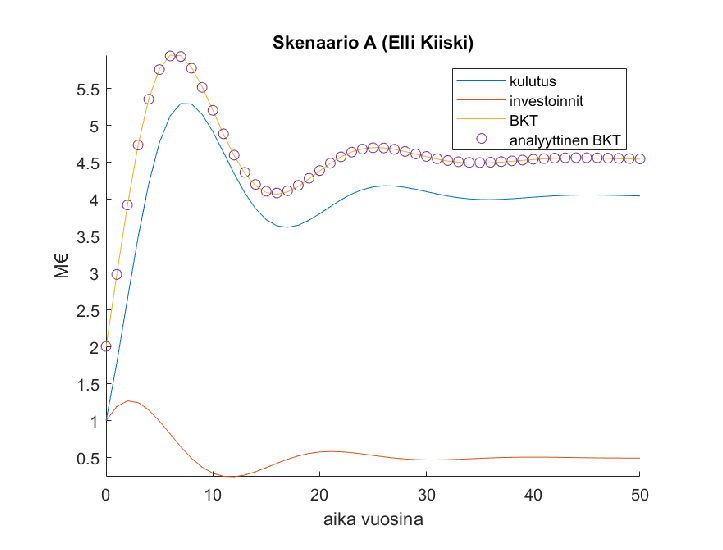
\includegraphics[width= 75mm]{kuva2-skenaarioA.eps}
    \caption{Skenaario A päätyy tasapainoon.}
    \label{sA}
\end{figure}

\begin{figure}
    \centering
    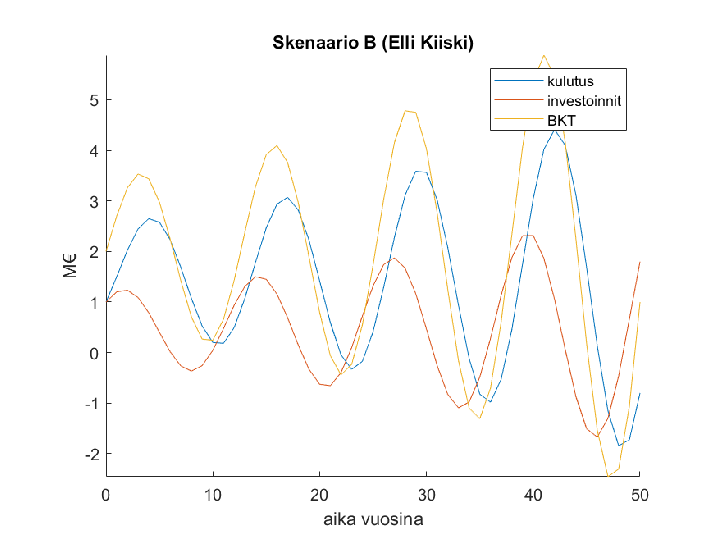
\includegraphics[width= 75mm]{kuva3-skenaarioB.eps}
    \caption{Skenaario B jatkaa heittelehtimistä.}
    \label{sB}
\end{figure}

\begin{figure}
    \centering
    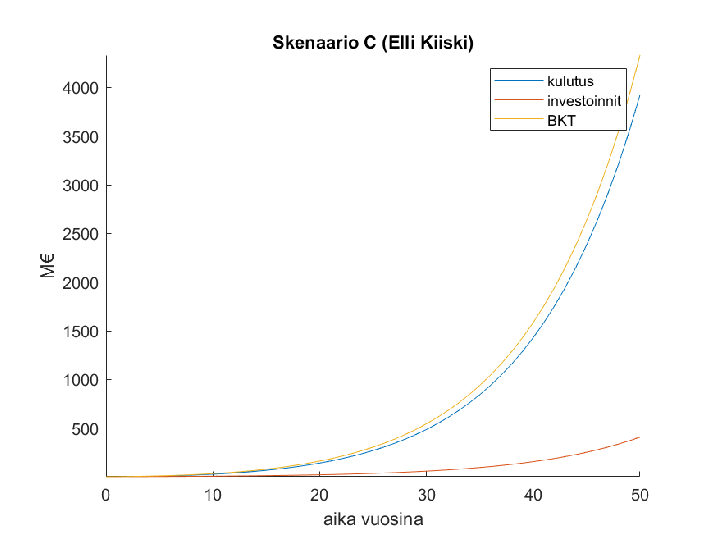
\includegraphics[width= 75mm]{kuva3-skenaarioC.eps}
    \caption{Skenaario C kasvaa exponentiaalisesti.}
    \label{sC}
\end{figure}

\subsection{Analyyttinen ratkaisu}

On väitetty, että skenaariolle A on olemassa analyyttinen ratkaisu ja se on muotoa $y_a(t)=k_1{r_1}^t+k_2{r_2}^t+c$, missä $k_1 = -1.27 + 0.98i$, $k_2 = -1.27 - 0.98i$, $r_1 = 0.84 - 0.29i$, $r_2 = 0.84 + 0.29i$ ja $c = 4.55$.

Tutkitaan väitteen paikkansapitävyyttä määrittelemällä ratkaisua vastaava funktio ja testaamalla sitä samaisella $50$ vuoden ajanjaksolla, kuin aiemmin skenaarion A simuloinnissa.

\clearpage

Määritellään yhtälöä vastaava funktio.

\begin{lstlisting}
function y = bkt(years)
% alkuarvot
k1 = -1.27 + 0.98i
k2 = -1.27 -0.98i
r1 = 0.84 - 0.29i
r2 = 0.84 + 0.29i
c = 4.55
% itse ratkaisu
y = k1 * r1.^years + k2 * r2.^years + c
\end{lstlisting}

Kun piirretään funktion arvoja skenaarion A kuvaajan päälle (komennolla \texttt{scatter(t, bkt(t))}) huomataan, että pisteet asettuvat mitä siisteimmin BKT-käyrälle, kuten kuvassa \ref{sA} näkyy. Se tarkoittaa tietenkin sitä, että analyyttinen ratkaisu on aivan oikea, ainakin tarvittavalla tarkkuudella.

\end{document}